\documentclass[a4paper, oneside, final]{memoir}
\usepackage[T1]{fontenc}
\usepackage[utf8]{inputenc}
\usepackage[british]{babel}
\usepackage{amsmath}
\usepackage{amsthm}
\usepackage{ifthen}
\usepackage{verbatim}

% bedre orddeling Gør at der som minimum skal blive to tegn på linien ved
% orddeling og minimum flyttes to tegn ned på næste linie. Desværre er værdien
% anvendt af babel »12«, hvilket kan give orddelingen »h-vor«.
\renewcommand{\britishhyphenmins}{22} 

% Fix of fancyref to work with memoir. Makes references look
% nice. Redefines memoir \fref and \Fref to \refer and \Refer.
% \usepackage{refer}             %
% As we dont really have any use for \fref and \Fref we just undefine what
% memoir defined them as, so fancyref can define what it wants.
\let\fref\undefined
\let\Fref\undefined
\usepackage{fancyref} % Better reference. 

\usepackage{pdflscape} % Gør landscape-environmentet tilgængeligt
\usepackage{fixme}     % Indsæt "fixme" noter i drafts.
\usepackage{hyperref}  % Indsæter links (interne og eksterne) i PDF

\usepackage[format=hang]{caption,subfig}
\usepackage{graphicx}
\usepackage{stmaryrd}
\usepackage{amssymb}
\usepackage{listings}
\usepackage{ulem} % \sout - strike-through
\usepackage{tikz}

%\renewcommand{\ttdefault}{txtt} % Bedre typewriter font
% \usepackage[sc]{mathpazo}     % Palatino font
%\renewcommand{\rmdefault}{urw-garamond} % Garamond
%\usepackage[urw-garamond]{mathdesign}

% \overfullrule=5pt
% \setsecnumdepth{part}
\setcounter{secnumdepth}{1} % Sæt overskriftsnummereringsdybde. Disable = -1.
\setlength{\parskip}{0.25in}

\title{Statistical Methods for Machine Learning\\Case 2}

\author{Troels Henriksen (athas@sigkill.dk) \\ Daniel Fairchild
  (daniel.fairchild@gmail.com)}

\date{\today}
\pagestyle{plain}

\newcommand{\nfrac}[2]{\frac{\displaystyle{#1}}{\displaystyle{#2}}}

\begin{document}

\maketitle

We have never used R before, so for the novelty, that is the language
we have decided to use for this assignment.

\section*{Question 1.1}

The code for this question is in \texttt{src/1112.R}.  The
pseudoinverse function had to be written from scratch, as we could not
find the library supposed to contain it.  We obtained the following
results.

\begin{tabular}{|l|r|}
  \textbf{Selection} & \textbf{RMS error} \\\hline
  1 & 4.944719 \\\hline
  2 & 6.880314
\end{tabular}

Selection 1 appears to have the smaller error compared to the true
results, which is expected as its model incorporates more measurements
than selection 2.  While body measurements are probably only slightly
independent, adding more still constitutes a net information increase.
\newpage
\section*{Question 1.2}

The code for this question is in \texttt{src/1112.R}.

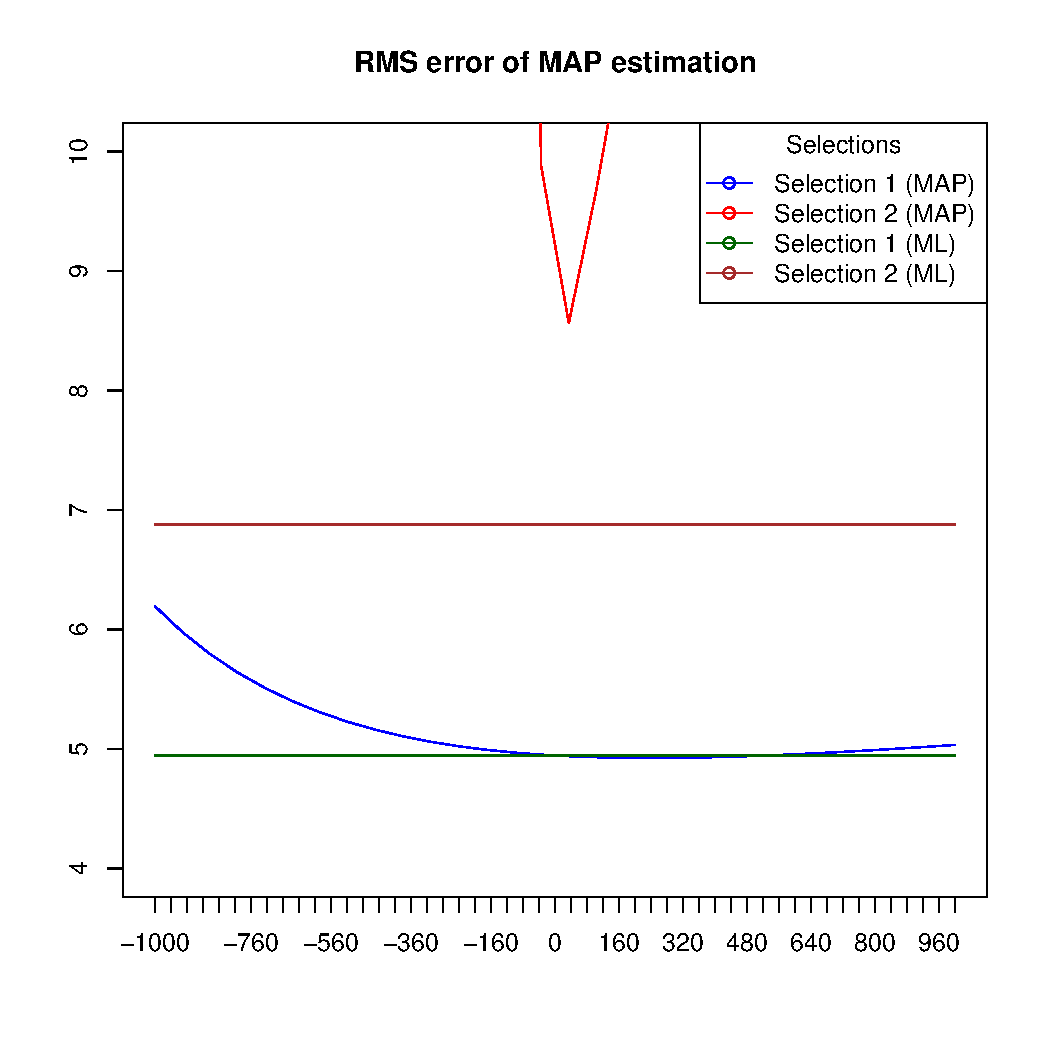
\includegraphics[width=10cm]{img/question12-plot.pdf}

Below is a close-up of the ML estimate and the MAP estimate.

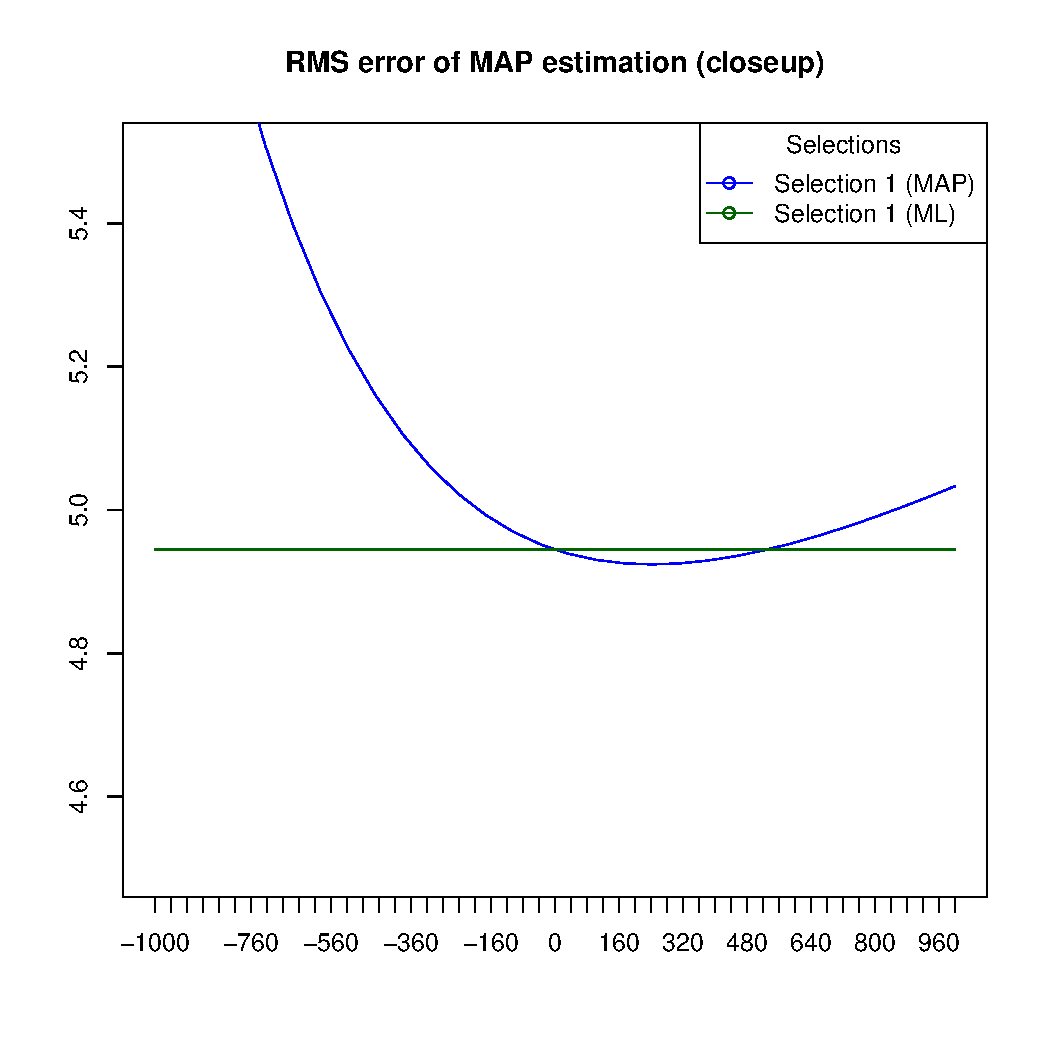
\includegraphics[width=10cm]{img/question12-plot-b.pdf}

We see that the MAP estimate has a slightly smaller error when the
prior precision is in the interval from roughly 0 to 500.

\end{document}
